\documentclass[19pt]{article}

\usepackage{arxiv}
\usepackage{makeidx}
\usepackage{fancyhdr}

\usepackage[utf8]{inputenc} % allow utf-8 input
\usepackage[T1]{fontenc}    % use 8-bit T1 fonts
\usepackage{hyperref}       % hyperlinks
\usepackage{url}            % simple URL typesetting
\usepackage{booktabs}       % professional-quality tables
\usepackage{graphicx}
\usepackage{amsfonts}       % blackboard math symbols
\usepackage{amsmath}
\usepackage{nicefrac}       % compact symbols for 1/2, etc.
\usepackage{microtype}      % microtypography
\usepackage{lipsum}

\pagestyle{fancy}
\title{AI in Medicine : Segmentation of Lymph tissues and localization of Cancer cells}


\author{
  Spandan Ghosh\thanks{Use footnote for providing further
    information about author (webpage, alternative
    address)---\emph{not} for acknowledging funding agencies.} \\
    Department of \emph{Electronics and Communication Engineering}\\
  Institute of Engineering \& Management\\
  Kolkata, India \\
  \texttt{spandanghosh2@gmail.com} \\
}
\begin{document}

\maketitle

\begin{abstract}
    Artificial Intelligence has been setting the benchmark for almost all commercial and research fields. Since the rapidly growing popularity of these approaches now draw the interests of the people in the resepective fields of application, we now define state of the art benchmarks with respect to how well several networks perform in different fields. Medical Imaging and the analysis of these images are no different. The polished techniques in Digital Image Processing such as the various filters, transforms, thresholding techniques have already been in use to reduce redundant human work when these techniques can perform pattern recognition for trivial, repititive tasks. The effect of the evolution of Deep Learning has allowed the learning of complex convolution filters using Convolutional Neural Networks(CNNs) which now permit the detection of intricate patterns and segmenting them to such an extent that these now become more efficient than the human eye in several cases. Medical Images however, post various challenges that are usually absent in other applications of Deep Learning in Computer Vision. 

    The first and primary issue is the quantity of data available. The amount of data available is nowhere close to the other real world applications such as classification of cusines by their snapshots. Moreover, medical images cannot be readily scraped or taken from the real world. Taking the problem at hand, one cannot simply step out into the world and acquire scanned and labelled images of Lymph Tissues. Their aquisition depends on Medical Institutions. Furthermore, the process of capturing, labelling, processing and releasing such a dataset is difficult and requires specialized attention from medical professionals. The second issue is that this, combined with the fact that expensive equipment may be required for their collection makes the process expensive.

    Segmentation adds another complexity:\textbf{The complexity of effort}. Segmentation involves a pixel to pixel mapping between the input and an output. Every single tissue sample image needs to be segmented by a medical expert for us to train an algorithm to do so automatically on other images. This process is tedious. In this project, along with reviewing certain approaches of interest, I am going to achive the a segmentation map on the input image without using a segmentation levels and am also going to discuss some alternative methods in which the above claimed can be achieved and when and where which should be preferred.
    
\keywords{Semantic Segmentation\and Medical Image Analysis \and Associative Networks \and Deep Learning}
\end{abstract}
\newpage
    \tableofcontents
\newpage
% keywords can be removed



\section{Introduction}
The upsurge in the dominance of Deep Learning in defining the Statei-of-the-Art in a great variety of fields. Both Research and Industrial organizations all over the world are on a lookout to capitalize on the edge provided by Deep Learning and to leverage an increase in performance or profit in accordance with the goals of the organization. With data being in abundance in this digital age and the greatly evolved compute capacity with the rise of GPUs (Graphical Processing Units), the tedious and compute hungry processing of training models on particular datasets has become easier and practically feasable.

\subsection{Motivation}
There has been a huge upsurge in the replacement of tedious and laborious work with algortihms to automate the process. Segmentation is no different. Segmentation is the process of reconstruction of an input image as the output image with certain pixels of the image highlighted or labelled to be of a particular class or to have a particular property. In Medical Imaging, this is quite often required in the highlighting of infected regions or affected areas in cells or scans. Before getting into the approaches in Digital Image Processing and Deep Learning to solve such problems, let us have a look at some typical segmentated images.

\begin{center}
    \begin{figure}[!h!t!b]
        \centerline{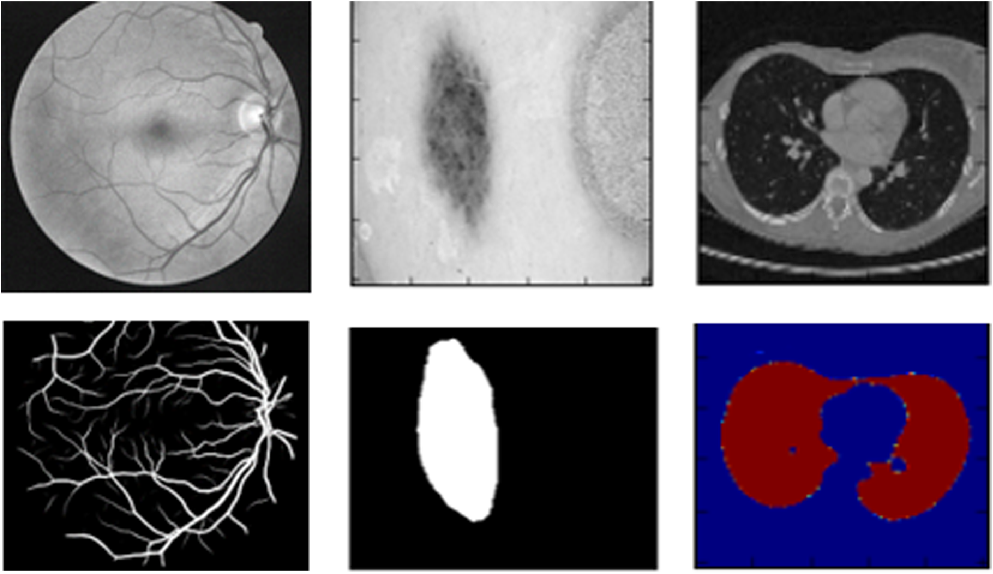
\includegraphics[width=105mm,height=65mm]{images/segs.png}}
        \caption{Some Segmented images : Row-1 has the input images and row 2 has the output images also known as the segmented images or the segmentation maps}
        \label{fig:1}
    \end{figure}
\end{center}

Segmentation is not limited to the world of medical prognosis. It is applicable in several fields of interest such as Handwriting analysis as seen in Kaur et. al.\cite{kour2014real}. The usual idea behind segmentation would be to design a mathematical function that proposes a mapping between input and output pixels. As seen in Fig. \ref{fig:1}, the left-most image is one that segments the retinal vesicles of the eye. Such a work would require constant supervision and analysis of such images manually by medical professionals as such a work requires a degree of domain knowledge and expertise.

This problem is one typical area where we would want to apply Image Processing to either independently solve the problem or to make the job easier by minimizing the human sipervision involved. The motivation as such, behind my analysis of approaches and the development of the project is the explotation of data to learn functions that map from the input image to the output image. However, such a task requires data in such a format that every input image has a corresponding output image in the dataset and this needs to be prepared as the dataset by the said professionals. 

This project shall deal with a detailed comparative analysis on several different approaches on that are used in Semantic Segmentation but also discuss the main process under consideration where we DO NOT have to use segmentation data but we can still Localize the affected areas simply from the available data. This project shall be beneficial for the localization of cells with or without segmentation data and if segmentation data is available, the comparative analysis shall help in the choice of approach as will be beneficial for the project. 

\subsection{Objective}
The Objective of this project is to achieve the localization of cancerous cells in slides containing lymph tissues in general. The specific problem we shall be dealing with is the identification of metastatic tissues in the histopathelogical scans of lymph node sections. 

\begin{center}
    \begin{figure}[!h!t!b]
        \centerline{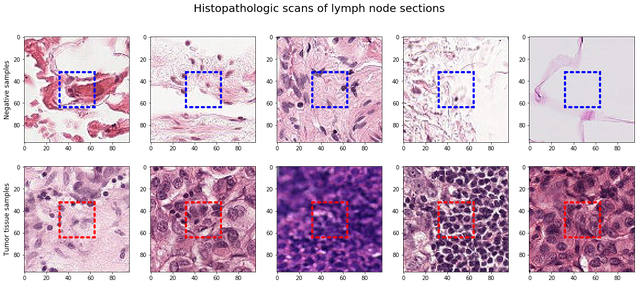
\includegraphics[width=105mm,height=65mm]{images/metastases.png}}
        \caption{The cells and a certain box showing the areas of possible interest}
        \label{fig:2}
    \end{figure}
\end{center}

\begin{center}
    \begin{figure}[!h!t!b]
        \centerline{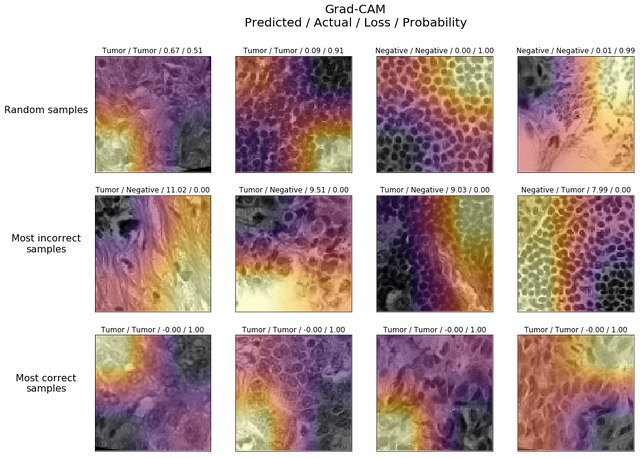
\includegraphics[width=105mm,height=65mm]{images/gradcam.png}}
        \caption{Gradcam or the regions in the input image that most affect the output in the image}
        \label{fig:3}
    \end{figure}
\end{center}

\newpage
\bibliographystyle{unsrt}  

\bibliography{references}  %%% Remove comment to use the external .bib file (using bibtex).
%%% and comment out the ``thebibliography'' section.


%%% Comment out this section when you \bibliography{references} is enabled.

\end{document}
